\documentclass[tikz,border=8pt]{standalone}
\usepackage{tikz}
\usepackage{fontspec}
\setmainfont{DejaVu Sans}
\setsansfont{DejaVu Sans}
\usetikzlibrary{arrows.meta, positioning, shapes.geometric, calc, fit, backgrounds}
\begin{document}
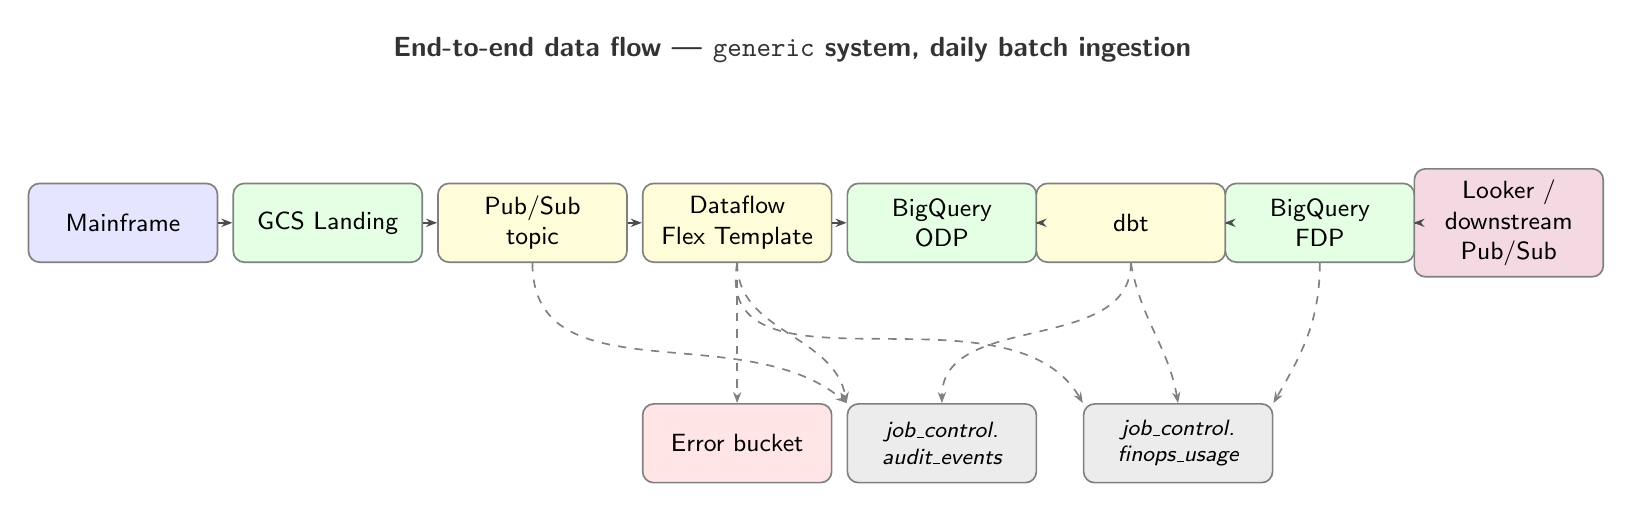
\begin{tikzpicture}[
  font=\sffamily\small,
  every node/.style={font=\sffamily\small},
  box/.style={draw=black!50, line width=0.6pt, rounded corners=4pt, minimum width=2.4cm, minimum height=1cm, align=center, inner sep=4pt},
  src/.style={box, fill=blue!10},
  storage/.style={box, fill=green!10},
  compute/.style={box, fill=yellow!15},
  output/.style={box, fill=purple!15},
  control/.style={box, fill=gray!15, font=\sffamily\footnotesize\itshape},
  err/.style={box, fill=red!10},
  arrow/.style={-{Stealth[length=4pt]}, line width=0.6pt, draw=black!70},
  dashed-arrow/.style={arrow, dashed, draw=black!50},
  caption/.style={font=\sffamily\footnotesize, text=black!60}
]

% Title
\node[font=\sffamily\normalsize\bfseries, text=black!80] (title) at (8.5,2.2)
  {End-to-end data flow --- \texttt{generic} system, daily batch ingestion};

% === MAIN SPINE (left to right) ===
\node[src]      (mf)  at (0,0)     {Mainframe};
\node[storage]  (gcs) at (2.6,0)   {GCS Landing};
\node[compute]  (ps)  at (5.2,0)   {Pub/Sub\\topic};
\node[compute]  (df)  at (7.8,0)   {Dataflow\\Flex Template};
\node[storage]  (odp) at (10.4,0)  {BigQuery\\ODP};
\node[compute]  (dbt) at (12.8,0)  {dbt};
\node[storage]  (fdp) at (15.2,0)  {BigQuery\\FDP};
\node[output]   (con) at (17.6,0)  {Looker /\\downstream\\Pub/Sub};

% Spine arrows
\draw[arrow] (mf)  -- (gcs);
\draw[arrow] (gcs) -- (ps);
\draw[arrow] (ps)  -- (df);
\draw[arrow] (df)  -- (odp);
\draw[arrow] (odp) -- (dbt);
\draw[arrow] (dbt) -- (fdp);
\draw[arrow] (fdp) -- (con);

% === CONTROL-PLANE BOXES (below spine) ===
\node[err]     (ebkt) at (7.8,-2.8)  {Error bucket};
\node[control] (aud)  at (10.4,-2.8) {job\_control.\\audit\_events};
\node[control] (fin)  at (13.4,-2.8) {job\_control.\\finops\_usage};

% Dashed arrows to error bucket
\draw[dashed-arrow] (df.south) -- (ebkt.north);

% Dashed arrows to audit_events
\draw[dashed-arrow] (df.south)  to[out=-90,in=100] (aud.north west);
\draw[dashed-arrow] (dbt.south) to[out=-90,in=90] (aud.north);
\draw[dashed-arrow] (ps.south)  to[out=-90,in=140] (aud.north west);

% Dashed arrows to finops_usage
\draw[dashed-arrow] (df.south)  to[out=-100,in=120] (fin.north west);
\draw[dashed-arrow] (dbt.south) to[out=-80,in=100]  (fin.north);
\draw[dashed-arrow] (fdp.south) to[out=-90,in=60]   (fin.north east);

\end{tikzpicture}
\end{document}
